\begin{frame}[fragile, shrink=50]
  \frametitle{Hyperelasticity}

  \vspace{1cm}

  \begin{columns}

    \begin{column}{0.5\textwidth}
      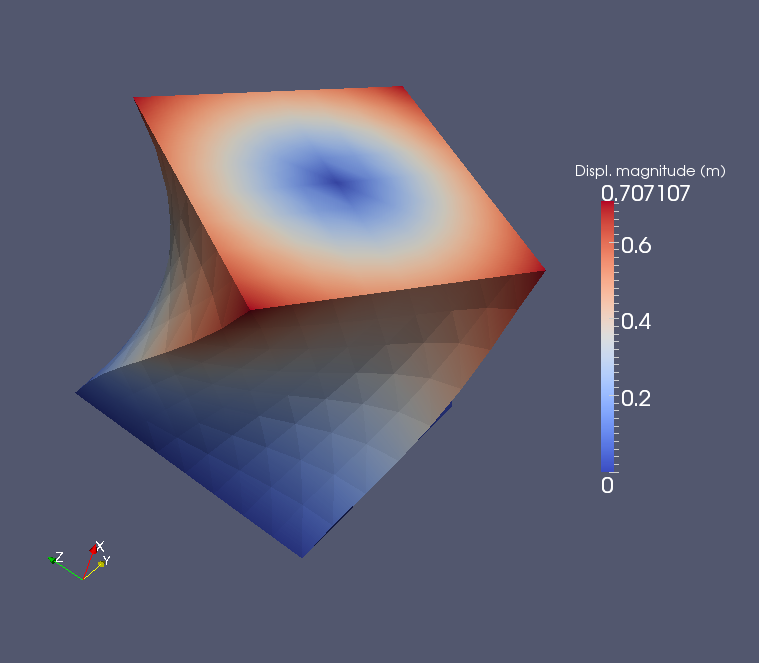
\includegraphics[width=\textwidth]{png/twistedcube.png}
    \end{column}

    \begin{column}{0.5\textwidth}
      \begin{python}
from fenics import *

mesh = UnitCubeMesh(24, 16, 16)
V = VectorFunctionSpace(mesh, "Lagrange", 1)

left =  CompiledSubDomain("(std::abs(x[0])       < DOLFIN_EPS) && on_boundary")
right = CompiledSubDomain("(std::abs(x[0] - 1.0) < DOLFIN_EPS) && on_boundary")

c = Expression(("0.0", "0.0", "0.0"), degree=0)
r = Expression(("0.0", 
"0.5*(y0+(x[1]-y0)*cos(t)-(x[2]-z0)*sin(t)-x[1])",
"0.5*(z0+(x[1]-y0)*sin(t)+(x[2]-z0)*cos(t)-x[2])"),
y0=0.5, z0=0.5, t=pi/3, degree=3)
bcl = DirichletBC(V, c, left)
bcr = DirichletBC(V, r, right)
bcs = [bcl, bcr]
v  = TestFunction(V)
u  = Function(V) 
B  = Constant((0.0, -0.5, 0.0))
T  = Constant((0.1,  0.0, 0.0))
I = Identity(V.cell().d)
F = I + grad(u)
Ic = tr(F.T*F)
J  = det(F)
E, nu = 10.0, 0.3
mu, lmbda = Constant(E/(2*(1 + nu))), Constant(E*nu/((1 + nu)*(1 - 2*nu)))
psi = (mu/2)*(Ic - 3) - mu*ln(J) + (lmbda/2)*(ln(J))**2
Pi = psi*dx - dot(B, u)*dx - dot(T, u)*ds
F = derivative(Pi, u, v)

solve(F == 0, u, bcs) 
plot(u, interactive=True, mode="displacement")
      \end{python}
    \end{column}
  \end{columns}

  % Compensate for scaling
  \huge

  \reference{H. Narayanan}
            {A computational framework for nonlinear elasticity}
            {2011}

\end{frame}
